\begin{block}{Agents}
    \begin{itemize} 
        \item The state of the agent can vary depending on the evolution of the simulation between: \textbf{susceptible}, \textbf{infected}, \textbf{notified}, \textbf{quarantined}.
        \item \textbf{Normally}, the target position of an agent changes randomly or can be manually imposed.
        \item An infected agent can \textbf{transmit} the disease to a normal agent with a given probability and according to a selected proximity range.
        \item If the agent is \textbf{infected}, he can exhibit symptoms with a given probability and therefore the target will become going to his diagnostician.
        \item If the agent is \textbf{notified}, the target immediately becomes going to his diagnostician.
        \item If the agent is \textbf{quarantined}, he cannot obviously move.
    \end{itemize}
\end{block}

\centering
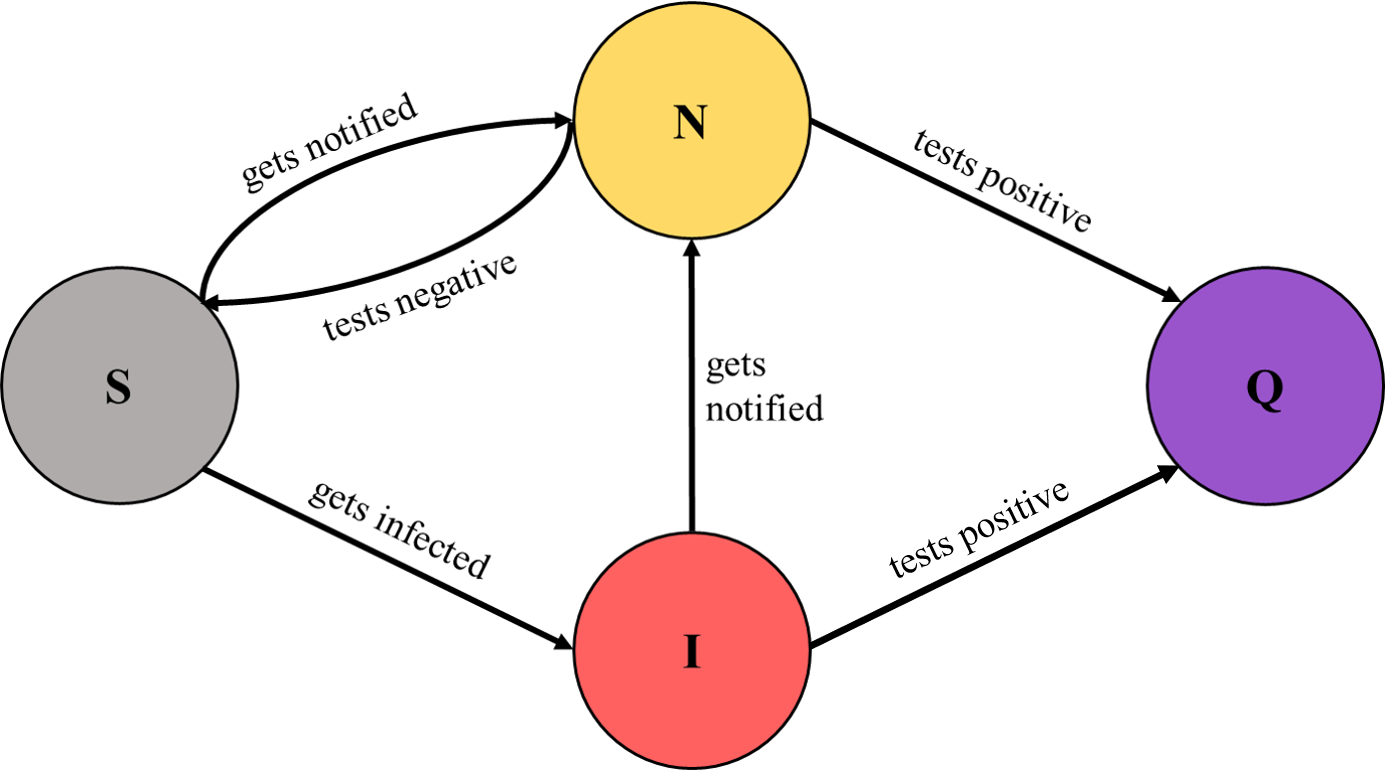
\includegraphics[width=0.4\linewidth]{images/statuses.png}
